

\begin{frame}{\ft{Intercepting Hyperlinks}}

\doubleFrame{With Re-PDF, Matterport hyperlinks can 
	then be \curlyquote{intercepted} --- that is, rather 
	than directing users to a web page, 
	the Re-PDF viewer can load specialized windows 
in accordance with 
	the user's current location in the virtual tour.}

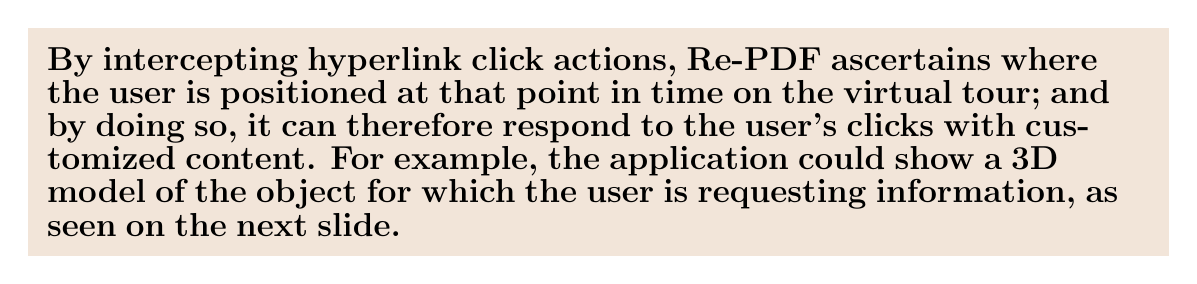
\begin{tikzpicture}
\nodeincludegraphicsTR{2.7cm}{2cm}{screenshots/ss-vt4.png}

 \node [anchor=west,fill=brown!20!white,inner sep=7, text width=14cm]
  (longnote) at (5.5,7) {%  %{\color{rb!85!red}{
  {\cframedbox{\large \textbf{By intercepting hyperlink click actions, 
  Re-PDF ascertains where the user is positioned at that point in 
  time on the virtual tour; and by doing so, 
  it can therefore respond 
  to the user's clicks with customized content.  For \makebox{example}, the 
  application could show a 3D model 
  of the object for which the user is requesting information, as 
  seen on the next slide.}}}};

\end{tikzpicture}


\end{frame}

